\subsection{Огляд функції пошуку маршрутів}
\label{subsec:route-management-subsection}

За допомогою функції пошуку маршруту користувачі можуть ввести початкову та кінцеву зупинки, щоб розпочати процес пошуку. Додаток використовує передові алгоритми для розрахунку найефективніших і найшвидших маршрутів на основі різних факторів, таких як відстань, час у дорозі та час очікування.

Результат пошуку відображається в чіткій та організованій. Маршрут супроводжується детальною інформацією, включаючи приблизний час у дорозі, відстань та покрокові вказівки.

Надаючи комплексну та зручну функцію пошуку маршрутів, застосунок має на меті спростити процес пошуку та навігації оптимальних маршрутів. Незалежно від того, чи користувачі їдуть на роботу, чи досліджують нове місто, чи планують подорож, вони можуть покластися на функцію пошуку маршрутів, яка надасть їм точні, ефективні та надійні варіанти маршрутів.

Пошук маршруту для користувача починається зі сторінки для вводу даних пошуку. На ній користувач може ввести початкову зупинку та кінцеву зупинку, а також бажаний час відправлення.

\begin{figure}[!htp]
	\centering
	
\includegraphics[scale=0.3]{content/chapters/4-results/assets/img/example1_search.png}
	\caption{Сторінка пошуку маршруту}
	\label{fig:search_page}
\end{figure}


Після вводу даних для пошуку, користувач натискає кнопку ``Знайти маршрут''. Застосунок оброблює введені дані, знаходить маршрут та відображає його.

\begin{figure}[!htp]
	\centering
	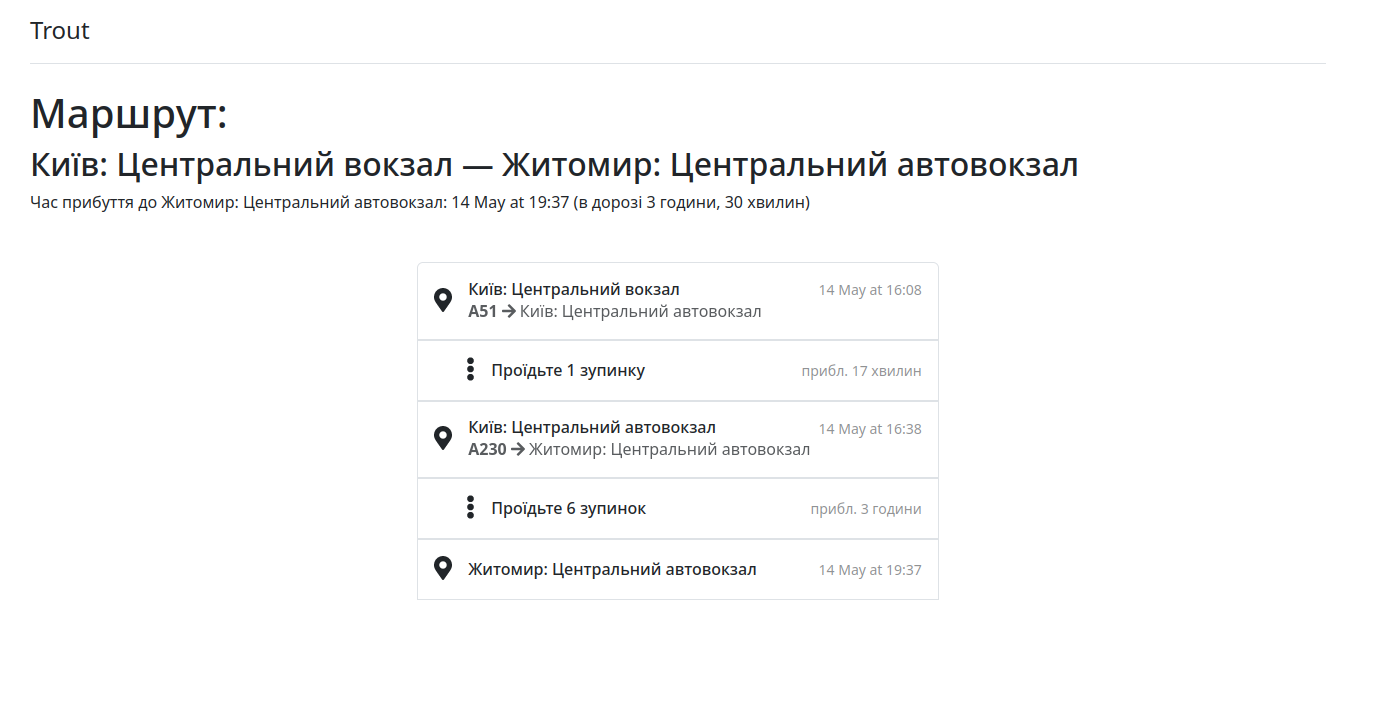
\includegraphics[scale=0.3]{content/chapters/4-results/assets/img/example1_result.png}
	\caption{Сторінка зі знайденим маршрутом}
	\label{fig:route_page}
\end{figure}


Користувач також може переглядати деталі про маршут та зупинки, які входять в знайдений маршрут.

\begin{figure}[!htp]
	\centering
	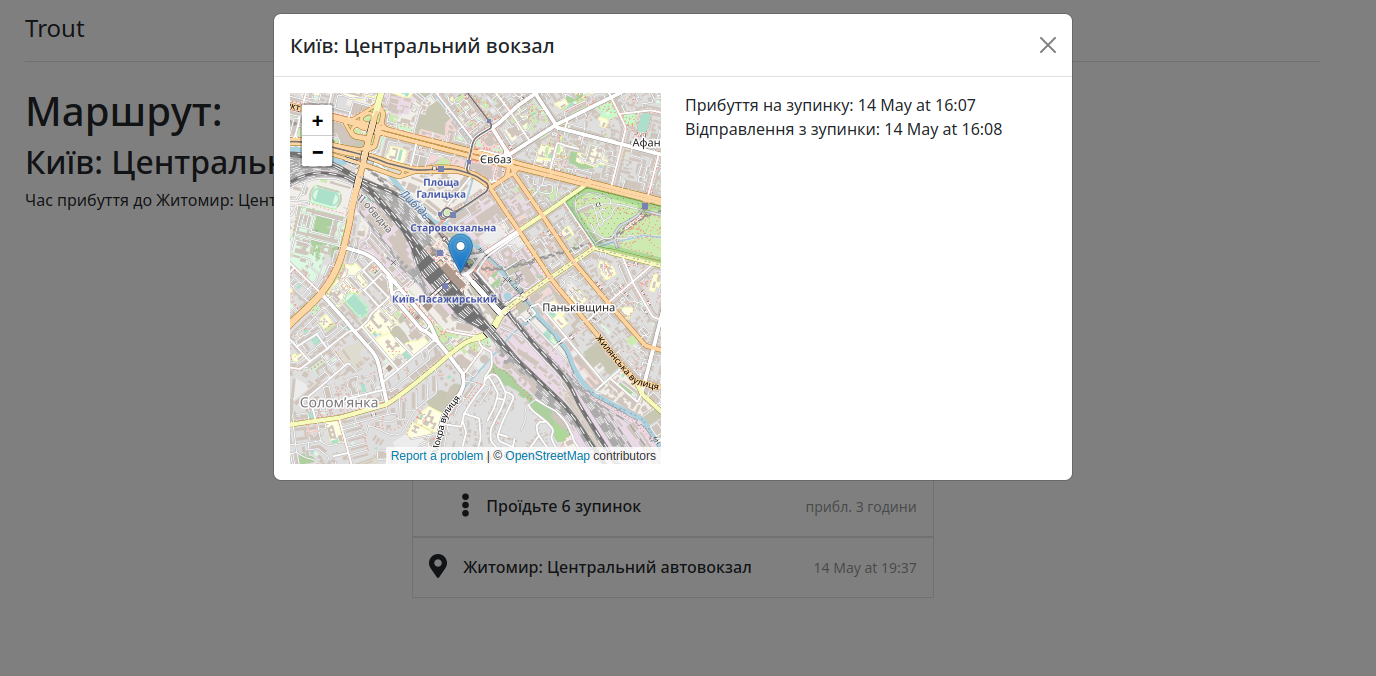
\includegraphics[scale=0.3]{content/chapters/4-results/assets/img/example_station.png}
	\caption{Перегляд деталей про зупинку}
	\label{fig:stop_details_page}
\end{figure}

\begin{figure}[!htp]
	\centering
	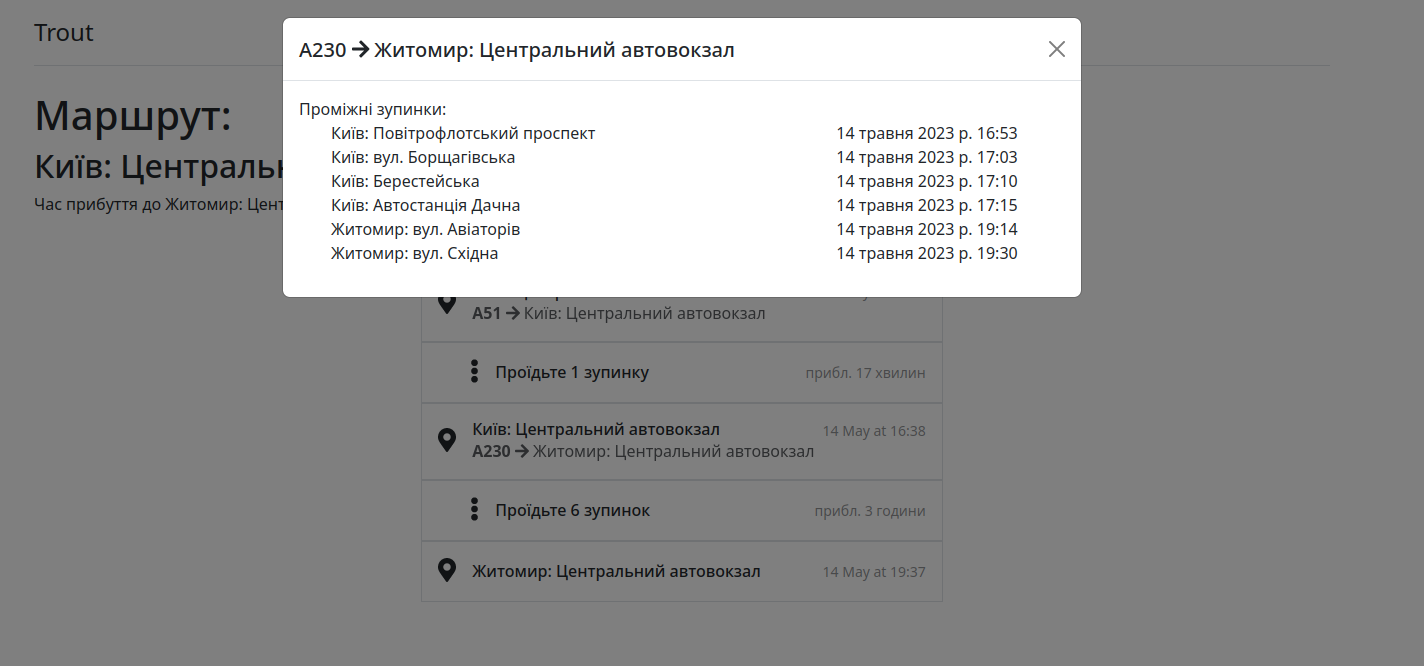
\includegraphics[scale=0.3]{content/chapters/4-results/assets/img/example_stops.png}
	\caption{Перегляд деталей про маршрут}
	\label{fig:route_details_page}
\end{figure}
